%to have line numbers
%\RequirePackage{lineno}
\documentclass[10pt, letterpaper]{article}      
\usepackage[margin=.1cm,font=small,labelfont=bf]{caption}[2007/03/09]
%\usepackage{endnotes}
%\let\footnote=\endnote
\usepackage{setspace}
\usepackage{longtable}                        
\usepackage{anysize}                          
\usepackage{natbib}                           
%\bibpunct{(}{)}{,}{a}{,}{,}                   
\bibpunct{(}{)}{,}{a}{}{,}                   
\usepackage{amsmath}
\usepackage[% draft,
pdftex]{graphicx} %draft is a way to exclude figures                
\usepackage{epstopdf}
\usepackage{hyperref}                             % For creating hyperlinks in cross references

 
% \usepackage[margins]{trackchanges}

% \note[editor]{The note}
% \annote[editor]{Text to annotate}{The note}
%    \add[editor]{Text to add}
% \remove[editor]{Text to remove}
% \change[editor]{Text to remove}{Text to add}

%TODO make it more standard before submission: \marginsize{2cm}{2cm}{1cm}{1cm}
\marginsize{1cm}{1cm}{.5cm}{.5cm}%{left}{right}{top}{bottom}   
					          % Helps LaTeX put figures where YOU want
 \renewcommand{\topfraction}{1}	                  % 90% of page top can be a float
 \renewcommand{\bottomfraction}{1}	          % 90% of page bottom can be a float
 \renewcommand{\textfraction}{0.0}	          % only 10% of page must to be text

 \usepackage{float}                               %latex will not complain to include float after float

\usepackage[table]{xcolor}                        %for table shading
\definecolor{gray90}{gray}{0.90}
\definecolor{orange}{RGB}{255,128,0}

\renewcommand\arraystretch{.9}                    %for spacing of arrays like tabular

%-------------------- my commands -----------------------------------------
\newenvironment{ig}[1]{
\begin{center}
 %\includegraphics[height=5.0in]{#1} 
 \includegraphics[height=3.3in]{#1} 
\end{center}}

 \newcommand{\cc}[1]{
\hspace{-.13in}$\bullet$\marginpar{\begin{spacing}{.6}\begin{footnotesize}\color{blue}{#1}\end{footnotesize}\end{spacing}}
\hspace{-.13in} }

%-------------------- END my commands -----------------------------------------



%-------------------- extra options -----------------------------------------

%%%%%%%%%%%%%
% footnotes %
%%%%%%%%%%%%%

%\long\def\symbolfootnote[#1]#2{\begingroup% %these can be used to make footnote  nonnumeric asterick, dagger etc
%\def\thefootnote{\fnsymbol{footnote}}\footnote[#1]{#2}\endgroup}	%see: http://help-csli.stanford.edu/tex/latex-footnotes.shtml

%%%%%%%%%%%
% spacing %
%%%%%%%%%%%

% \abovecaptionskip: space above caption
% \belowcaptionskip: space below caption
%\oddsidemargin 0cm
%\evensidemargin 0cm

%%%%%%%%%
% style %
%%%%%%%%%

%\pagestyle{myheadings}         % Option to put page headers
                               % Needed \documentclass[a4paper,twoside]{article}
%\markboth{{\small\it Politics and Life Satisfaction }}
%{{\small\it Adam Okulicz-Kozaryn} }

%\headsep 1.5cm
% \pagestyle{empty}			% no page numbers
% \parindent  15.mm			% indent paragraph by this much
% \parskip     2.mm			% space between paragraphs
% \mathindent 20.mm			% indent math equations by this much

%%%%%%%%%%%%%%%%%%
% extra packages %
%%%%%%%%%%%%%%%%%%

\usepackage{datetime}


\usepackage[latin1]{inputenc}
\usepackage{tikz}
\usetikzlibrary{shapes,arrows,backgrounds}


%\usepackage{color}					% For creating coloured text and background
%\usepackage{float}
\usepackage{subfig}                                     % for combined figures

\renewcommand{\ss}[1]{{\colorbox{blue}{\bf \color{white}{#1}}}}
\newcommand{\ee}[1]{\endnote{\vspace{-.10in}\begin{spacing}{1.0}{\normalsize #1}\end{spacing}\vspace{.20in}}}
\newcommand{\emd}[1]{\ExecuteMetaData[/tmp/tex]{#1}} % grab numbers  from stata

%TODO before submitting comment this out to get 'regular fornt'
\usepackage{sectsty}
\allsectionsfont{\normalfont\sffamily}
\usepackage{sectsty}
\allsectionsfont{\normalfont\sffamily}
\renewcommand\familydefault{\sfdefault}

\usepackage[margins]{trackchanges}
\usepackage{rotating}
\usepackage{catchfilebetweentags}

\usepackage{abstract}
\renewcommand{\abstractname}{}    % clear the title
\renewcommand{\absnamepos}{empty} % originally center
%-------------------- END extra options -----------------------------------------
\date{{}\today}
\title{  % remember to have Vistula University!!
  The effect of social transfers and social capital on subjetive wellbeing of
elderly--are there cross-country differences?\footnote{This study was funded by grant \# 2016/21/B/HS4/03058 from
  Polish National Science Foundation (Narodowe Centrum Nauki).}
}
\author{
Adam Okulicz-Kozaryn\thanks{EMAIL: adam.okulicz.kozaryn@gmail.com
  \hfill I thank XXX.  All mistakes are mine.} \\
{\small Rutgers - Camden  and Vistula University}
}

\begin{document}

%%\setpagewiselinenumbers
%\modulolinenumbers[1]
%\linenumbers

\bibliographystyle{/home/aok/papers/root/tex/ecta}
\maketitle
\vspace{-.4in}
\begin{center}

\end{center}


\begin{abstract}
\noindent
\end{abstract}
\vspace{.15in} 
\noindent{\sc XXX TODO add to ebib as keyword PAPER-CODE-NAME and tag with ebib keywords 
}
\vspace{.25in} 

\begin{spacing}{1.4} %TODO MAYBE before submission can make it like 2.0
\rowcolors{1}{white}{gray90}

%  instead \ExecuteMetaData[../out/tex]{ginipov} do \emd{ginipov}

% \begin{figure}[H]
%  \includegraphics[height=3in]{../out/gov_res_trust.pdf}\centering\label{gov_res_trust}
% \caption{woo}
% \end{figure}


%TODO !!!! have input here aok_var_des


Recent CITE Rubia livability find spaital patterns in wellbeing across europe with
north west being most satisfied and south east least. \citet{fuentes17} find
that the relationship between binge drinking and SWB is moderated by region. In
present study we want to find out how the relationship of volunteering, social
transfers and SWB vary across countries. 

There have been many studies on cross-country differencs in SWB (eg mine about
eur and cite ruut) and about diff in volunteering (haski the one from oecd that
leszek emailed in dec2017 in word some writep), but no study on the varying
effect of volunteering and pensions on swb across countries. 
we build on $<$blind for peer review$>$  % socTraCocCap
just extend across countries
 



\citet{duda16} %sec7.3
review several studies using SHARE and finding similar
pattern: North is happier than South.

Welfare helps general population
\citep{radcliff01,pacek08b,pacek08r,radcliff13,aokJap14} and so it does help elderly
in Europe \citep{motel09,niedzwiedz14}. Importantantly, welfare was found not to
crowd out the helping among people \citep{motel05}. In fact there is evidence to
the contrary, the more welfare (and civil liberties), the more volunteering
\citep{hank10}.
%
There is however evidence, that familism \citep{banfield67}, or Southern
informal high level of relations and engagement within family networks tend to
crowd out the formal forms of engagment such as volunteering
\citep{kohli09,pichler07}. Being from Poland, we expect that similar mechanism may be at work in Eastern Europe.



We know that volunteering varies by country \citep[e.g.,][]{hank09}. This study
will focus on testing whether there is a varying effect from volunteering on SWB
by country. 

This study contnues a line of research focusing on cross-country comparisons
\citep{hank05,hank09}. We focus on subjective wellbeing as an consequence  of
volunteering; that is we are not interested here in antecdants of volunteering
neither in other consequences. 

Note, however, the goal of the present study is not to investigate what
predicts or affects volunteering cross nationally as in \citet{hank05,hank09},
but to examine the subsequent link, the link between volunterring and wellbeing cross-nationally.


have bar charts or tablesor key vars for each country, like in my earlier
cross=area paper s like one with mari or my earlier stuff for SIR

heck just redo overall paper broken down by country and again, have country in
rows and effects as 95 perc CI--there is some stata command for that

build on livability paper with rubia :)



Finally, we would like to test a proposition that effects differ across countries. % {For
  % instance, literature suggests that Northerners are more  satisfied with
  % social contacts \citep{bonsang12}.}and way more social transfers!
Perhaps, there are two clusters, North-Western and South-Eastern:\\
% Specifically, North-West is more individualistic (e.g., volunteering) and
% South-East is more collectivist (e.g., collectivist social capital and social transfers):\\ 

\noindent$H_3:$ Social transfers  will have
higher payoff in happiness in South-Eastern Europe; Volunteering will generate more
happiness in North-Western Europe.\\ %ee (mayble also south):lezy sie is sie



Finally, we expect large cross-national differences: what works in one
country may not work in another. Population aging in Europe is a fact, and
governments already grapple with spending pressures and budget deficits. What is
the best way to care about our seniors and ensure decent levels of wellbeing? We
hope to produce new knowledge in this area.  

\section{Literature}

Choi's environmental factors and structural factors such as region, urbanicity,
religion, life styles and social roles affect volunteering \citep[][cited in]{hank09}.
 We are inteested in finding whether similar factors can also affect the
 relationship between volunteering and wellbeing. 

Haski09 found rel between vol and swb strongest in countries with least of
it--not surpising--like educ in us--syates with fewest ppl taking sat like tx
highest score; in general these who go first those with greatest inclination, so
unfortunately increasing vol may have diminishing marginal returns

refer to and compare to 
visualizations--pretty cool by Morten Wahrendorf:
\url{http://www.wahrendorf.de/lifecourses/chrono.html}
\url{http://www.wahrendorf.de/lifecourses/map_1.html}


\section{Data}

Using the most recent wave 6--the adbantage that the very wide country coverage:
18 countries!

mostly copied from the other one

Here we take the perspective as in \citet{hank10} and look at three dimensions
of social capital (and 'productive aging') % hank calles them dimensions of
                                % productve aging, guess fine; but seems more
                                % accurate to say dimensions of soc cap!
\begin{itemize}
\item volunteering:  done voluntary or charity work
\item informal helping: provided help to family, friends or neighbors
\item caring: cared for a sick or disabled adult 
\end{itemize}

TODO: note the differenceL now volunteering in past XXX, earlier it was in past
XXX as in \citet{haski09}

\section{Results}

graphs: guess have a bar charts: volunteering and especially informal helping
like ghto---again as per ersa the idea is that there is cultuer: in south east
more familism! yes ! do talk about familism!!

have bar chart replicating tab2 and tab4 from hank05--disuss variaton in
informal help!

We also have ghto variable--the advantage--available for many cases (from
imputed dataset), but not really asmuch volunteering as rather helping and
assisting as opposed to voluntary taking part in community life; furthermore it
may point to unhappiness, at least unhappiness around as helping is probably
often induced by unhappiness of people who need help.  


CASP and life satisfaction correlate at .6, and while in general countries high
on one and hogh on the other one and low on one and on teh other one, there are
some notable differences shown in figure \ref{ls-casp-means}.

\begin{figure}[H]
 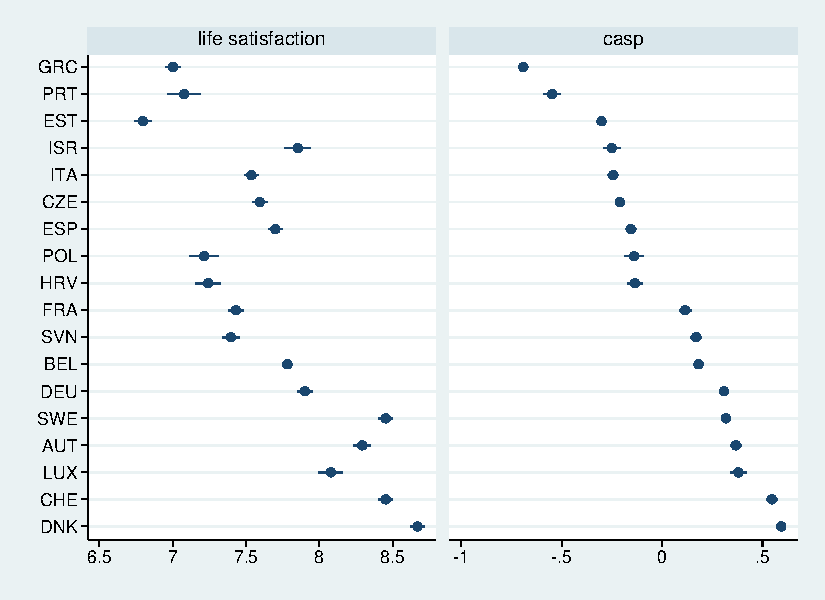
\includegraphics[height=3in]{tmp/ls-casp-means.pdf}\centering\label{ls-casp-means}
\caption{woo}
\end{figure}

%relating to lm ideas
So we also fins as in \citet{haski09} that highest volunteering is in Northern
counrties and lowest in Southern and effect differs by country


in fig \ref{reg-volCha}
so largest effect in south--interesting! guess the poorer the more vol matters!
same as in 1st paper !

\begin{figure}[H]
 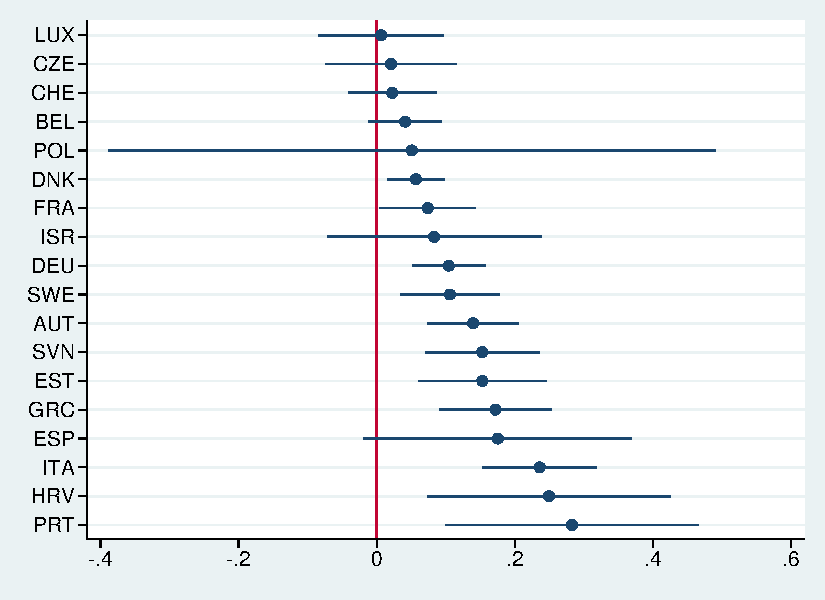
\includegraphics[height=3in]{tmp/reg-volCha.pdf}\centering\label{reg-volCha}
\caption{woo}
\end{figure}


\section{Discussion}

TODO add from ERSA as per culture etc etc

Volunteering is related to SWB. And many European countries have very low rates
of volunteering. So what are the practical implications? Volunteering could be
induced--there are many ways to activate this yet unused potential of idle
elderly \citep[e.g.,][]{atkinson2006mobilizing,henkin2006communities, butler2007civic,Butts,howgate2008increasing,zedlewski2007we}. And
there is a role for institutions of higher education to promote civic engagement
and community development in general, not only among the elderly. See, for instance,
initiatives at Rutgers-Camden \url{http://www.camden.rutgers.edu/civic-engagement}.
 Such initiatives could be copied by institutions of higher education in
 European countries with low engagment, such as Poland. 

% %table centered on decimal points:)
% \begin{table}[H]\centering\footnotesize
% \caption{\label{freq_im_god} importance of God}
% \begin{tabular} {@{} lrrrr @{}}   \hline 
% Item& Number & Per cent   \\ \hline
% 1(not at all)&    9,285&  9\\
% 2&    3,555&        3\\
% 3&    3,937&        4\\
% 4&    2,888&        3\\
% 5&    7,519&        7\\
% 6&    5,175&        5\\
% 7&    6,050&        6\\
% 8&    8,067&        8\\
% 9&    8,463&        8\\
% 10&   52,385&       49\\
% Total&  107,324&      100\\ \hline
% \end{tabular}\end{table}


% % Define block styles
% \tikzstyle{block} = [rectangle, draw, fill=black!20, 
%     text width=10em, text centered, rounded corners, minimum height=4em]
% \tikzstyle{b} = [rectangle, draw,  
%     text width=6em, text centered, rounded corners, minimum height=4em]
% \tikzstyle{line} = [draw, -latex']
% \tikzstyle{cloud} = [draw, ellipse,fill=black!20, node distance = 5cm,
%     minimum height=2em]
    
% \begin{tikzpicture}[node distance = 2cm, auto]
%     % Place nodes
%     \node [block] (lib) {liberalism, egalitarianism, welfare};
%     \node [block, below of=lib] (con) {conservatism, competition, individualism};
%     \node [cloud, right of=con] (ls) {well-being};
%     \node [block, below of=ls] (cul) {genes, culture};
%     \node [b, left of =lib, node distance = 4cm] (c) {country-level};
%     \node [b, left of =con,  node distance = 4cm] (c) {person-level};
%     % Draw edges
%     \path [line] (lib) -- (ls);
%     \path [line] (con) -- (ls);
%     \path [line,dashed] (cul) -- (ls);
% \end{tikzpicture}


%PUT THIS NOTE, polish and put to /root/author_what_data --ALWAYS
%stick here stuff as i run it!!! maybe comment out later...


TODO: have separate som-r.tex as opposed to having it below; and in paper say
see supplemetary material as opposed to see appendix!
 \section*{\Huge ONLINE APPENDIX}
% \textbf{[note: this section will NOT be a part of the final version of
%   the manuscript, but will be available online instead]} %hence everything below
%                                 %is organized byu section, not subsection
% !!!
% have most of the stuff outputted to online appendix:)--start with that and then
% select stuff to paper--have brief narrative describng patterns in online app too
% !!!

% \section*{Variables' definitions, coding, and distributions}
% \label{app_var_des}


% %\input{/tmp/a.tex} %aok_var_des

% % \begin{spacing}{.9}
% %   \begin{table}[H]\centering \caption{Summary statistics.} \label{sumSta} \begin{scriptsize} \begin{tabular}{p{1.8in}p{.5in}p{.5in}p{.5in}p{.5in}p{.5in}p{.5in}p{.5in}p{.5in}p{.5in}p{.5
% %             in}p{.5in}p{.5 in}}\hline
% %         \input{/tmp/aha2.tex}
% %          \end{tabular}\end{scriptsize}\end{table}
% % \end{spacing}

% % \begin{spacing}{.9}
% %   \begin{table}[H]\centering \caption{Correlation matrix.} \label{sumSta} \begin{scriptsize} \begin{tabular}{@{}
% %           p{1.2in} rrrrrrrrrrrrr @{}}\hline
% %         \input{/tmp/ahb2.tex}\hline
% %          \end{tabular}\end{scriptsize}\end{table}
% % \end{spacing}



% Table XXX shows variable distributions. If a variable has more than
% 10 categories it is classified into bins...

% %\input .... %TODO !!!! have input here histograms

% \section*{Additional Descriptive Statistics}
% \label{app_des_sta}

% %make sure i have [H] or h! ???
% % \begin{table}[H]
% % \caption{}
% % \centering
% % \label{}
% % \begin{scriptsize}
% % \input{../out/reg_c.tex}
% % \end{scriptsize}
% % \end{table}

volunteeringh and frq of volunteering are closely related in fig \ref{volCha-volChaOft-means}

\begin{figure}[H]
 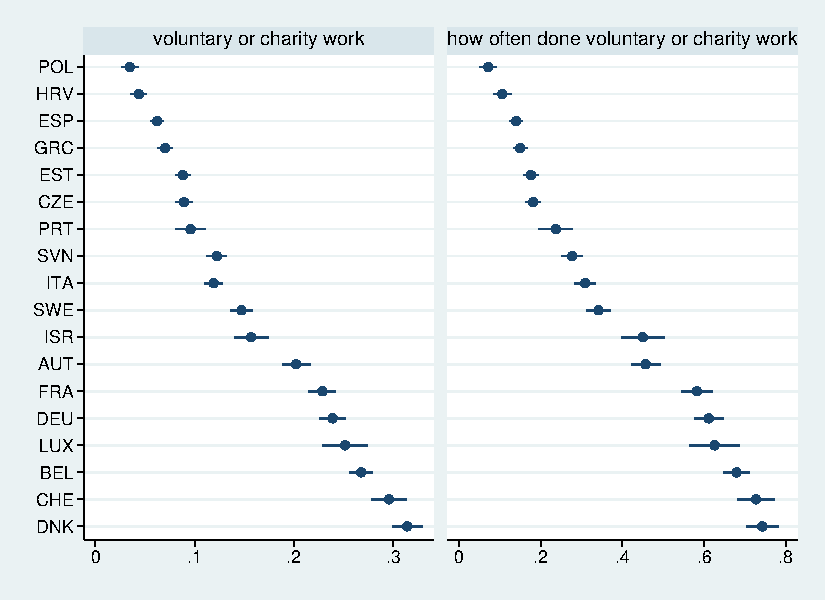
\includegraphics[height=3in]{tmp/volCha-volChaOft-means.pdf}\centering\label{volCha-volChaOft-means}
\caption{}
\end{figure}

the poorer the country, the more the pension matter in fig \ref{pen-means}

\begin{figure}[H]
 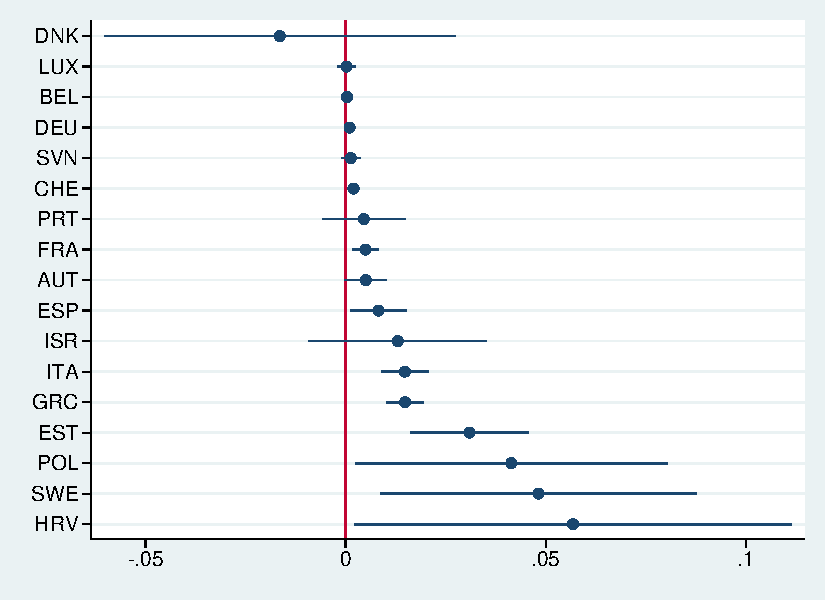
\includegraphics[height=3in]{tmp/pen-means.pdf}\centering\label{pen-means}
\caption{note: dropped CZE--it has some weird stange big value!}
\end{figure}


\begin{figure}[H]
 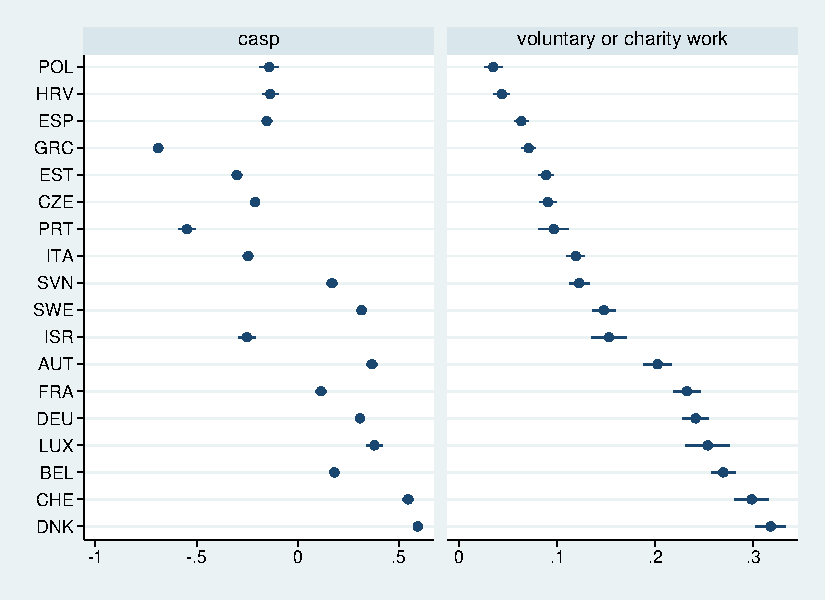
\includegraphics[height=3in]{tmp/casp-volCha-means.pdf}\centering\label{casp-volCha-means}
\caption{}
\end{figure}


\begin{figure}[H]
 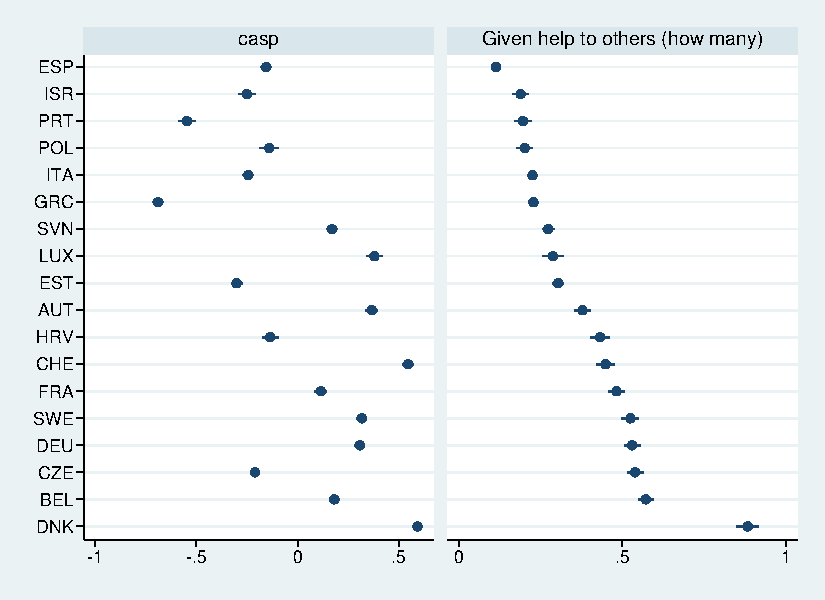
\includegraphics[height=3in]{tmp/casp-ghto-means.pdf}\centering\label{casp-ghto-means}
\caption{}
\end{figure}

\begin{figure}[H]
 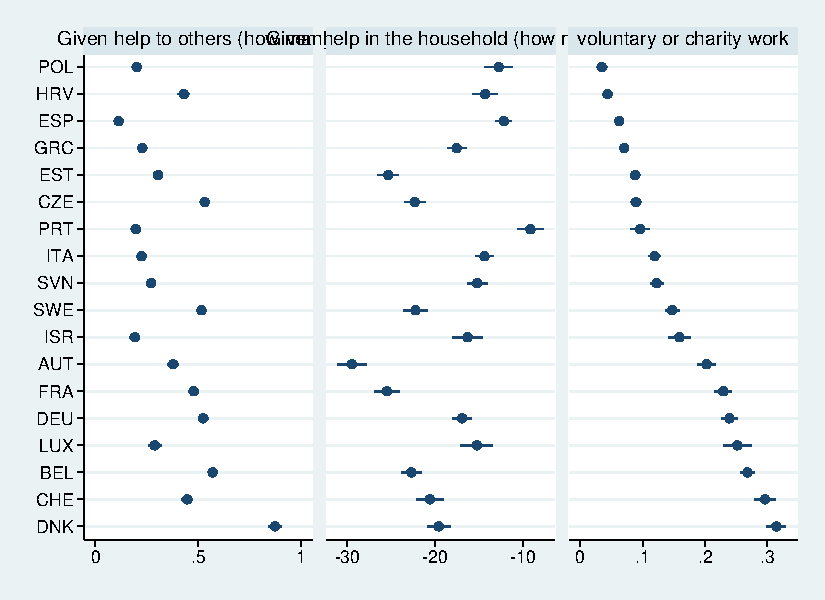
\includegraphics[height=3in]{tmp/ghto-ghih-volCha-means.pdf}\centering\label{ghto-ghih-volCha-means}
\caption{}
\end{figure}



%\newpage
%\theendnotes
\bibliography{/home/aok/papers/root/tex/ebib.bib,../tex-socTraSocCap/socTraSocCap.bib}



\end{spacing}
\end{document}
